\documentclass[11pt]{article}
\usepackage[utf8]{inputenc}
\usepackage[spanish,es-tabla]{babel}
\usepackage{amsmath,cancel}
\usepackage{amsfonts}
\usepackage{amssymb}
\usepackage{listings}
\usepackage{xcolor}
\usepackage{tabularx}
\usepackage{adjustbox}
\spanishdecimal{.}
\usepackage{graphicx}
\usepackage{float}
\usepackage[lmargin=2.5cm,rmargin=2.5cm,top=2.5cm,
bottom=2cm]{geometry}
\newcommand{\nombre}{Oscar}
\newcommand{\fecha}{9 de mayo del 2026}
\newcommand{\tituloPractica}{}
%%%%%%%%%%%%%%%%%%%%%%%%%%%%%%%%%%%%%%%%%%%%%%
\begin{document}
\begin{titlepage}
\begin{center}
\vspace*{2\baselineskip}
\hrule height 3pt
\vspace*{0.5\baselineskip}
{\Large \textbf{UNIVERSIDAD DE GUADALAJARA}}\\[0.1cm]
{\large \textbf{CENTRO UNIVERSITARIO DE CIENCIAS EXACTAS E INGENIER\'IAS}}
\vspace*{0.5\baselineskip}
\hrule
\vspace*{3\baselineskip}
\includegraphics[width=0.2\textwidth]{udg}
\vspace*{2\baselineskip}\\
{\large\textbf{ Algor\'itmos Bio-Inspirados \\ Msc. Rob\'otica e Inteligencia Artificial}
\vspace*{\baselineskip}\\
{\large Algoritmo 6 --- Algoritmo Gen\'etico N-Dimensional \vspace{1cm} \\
\begin{tabular}{p{4cm}p{8cm}}
\hline \hline
Nombre del alumno:  & Oscar Alberto Gallo Garc\'ia \\
C\'odigo del alumno:  & 218357704 \\
Profesor: & Dr. Carlos Alberto Lopez Franco \\
 \hline \hline
\end{tabular}
\vfill
\fecha
\end{center}
\newpage
\end{titlepage}

\tableofcontents
\newpage

\section{Resumen}

Se implement\'o el Algoritmo Gen\'etico (AG) con codificaci\'on binaria en $n$ dimensiones. Cada individuo codifica una soluci\'on candidata como una cadena de bits; los operadores gen\'eticos de selecci\'on por torneo, cruzamiento de un punto y mutaci\'on de bits con elitismo permiten evolucionar la poblaci\'on hacia regiones de mayor aptitud. Se evaluaron doce casos: minimizaci\'on y maximizaci\'on en 2 dimensiones con gr\'aficas de superficie y contorno, y minimizaci\'on y maximizaci\'on en 4 dimensiones.

\section{Metodolog\'ia}

Los Algoritmos Gen\'eticos son m\'etodos de b\'usqueda y optimizaci\'on inspirados en la evoluci\'on biol\'ogica. Operan sobre una poblaci\'on de soluciones candidatas representadas como cromosomas, a las que aplican operadores gen\'eticos para generar nuevas generaciones con mejores valores de aptitud.

\subsection{Codificaci\'on binaria}

Cada variable real $x_d \in [\ell_{\min},\ell_{\max}]$ se codifica con $b$ bits. La decodificaci\'on convierte el entero sin signo $k_d$ representado por los bits en el valor real:

\[
x_d = \ell_{\min} + k_d \cdot \frac{\ell_{\max} - \ell_{\min}}{2^b - 1}, \qquad k_d \in \{0,1,\ldots,2^b-1\}
\]

Un individuo de $n$ dimensiones tiene longitud de cromosoma $L = n \cdot b$ bits.

\subsection{Selecci\'on por torneo}

Se seleccionan $k = 3$ individuos al azar de la poblaci\'on; el de mayor aptitud (menor $f$ en minimizaci\'on) gana y se agrega a la poblaci\'on de padres. El proceso se repite hasta completar el tama\~no de la poblaci\'on:

\[
\text{ganador} = \arg\min_{i \in \mathcal{C}} f\!\left(\mathbf{x}_i\right), \qquad |\mathcal{C}| = k
\]

\subsection{Cruzamiento de un punto}

Dados dos padres $\mathbf{p}_1$ y $\mathbf{p}_2$ de longitud $L$, se elige un punto de corte $c \sim \mathcal{U}\{1,\ldots,L-1\}$ con probabilidad $p_c$:

\[
\mathbf{h}_1 = \mathbf{p}_1[0{:}c]\;\|\;\mathbf{p}_2[c{:}L], \qquad
\mathbf{h}_2 = \mathbf{p}_2[0{:}c]\;\|\;\mathbf{p}_1[c{:}L]
\]

Si no ocurre cruzamiento (probabilidad $1-p_c$) los hijos son copias de los padres.

\subsection{Mutaci\'on de bits}

Cada bit del cromosoma se invierte de forma independiente con probabilidad $p_m$:

\[
\text{bit}'_j =
\begin{cases}
1 - \text{bit}_j & \text{si } u_j < p_m,\quad u_j \sim \mathcal{U}(0,1) \\
\text{bit}_j     & \text{en caso contrario}
\end{cases}
\]

\subsection{Elitismo}

El mejor individuo de la generaci\'on $t$ (\'elite) se preserva sin modificaci\'on en la generaci\'on $t+1$, ocupando la primera posici\'on del nuevo arreglo. Esto garantiza que la aptitud del mejor no retroceda entre generaciones.

\subsection{Algoritmo gen\'etico}

\begin{enumerate}
    \item Inicializar la poblaci\'on: $\mathbf{x}_i \sim \mathcal{U}_{\{0,1\}}^{L}$ para $i = 1,\ldots,n_p$.
    \item Evaluar $f(\mathbf{x}_i)$ y determinar el individuo \'elite.
    \item Repetir hasta $t_{\max}$ generaciones:
    \begin{enumerate}
        \item Selecci\'on por torneo $\rightarrow$ $n_p$ padres.
        \item Cruzamiento por pares $\rightarrow$ $n_p$ hijos.
        \item Mutaci\'on bit a bit sobre cada hijo.
        \item Reemplazar primer hijo con el \'elite.
        \item Evaluar; actualizar \'elite si se encuentra mejor soluci\'on.
    \end{enumerate}
    \item Decodificar y retornar la mejor soluci\'on.
\end{enumerate}

\subsection{Par\'ametros}

\begin{table}[H]
\centering
\begin{tabular}{lcc}
\hline\hline
Par\'ametro & 2D & 10D \\
\hline
N\'umero de bits $b$              & 16   & 16   \\
$p_c$ (factor de cruzamiento)    & 0.85 & 0.85 \\
$p_m$ (factor de mutaci\'on/bit) & 0.01 & 0.01 \\
$n_p$ (tama\~no de poblaci\'on)  & 60   & 100  \\
Iteraciones m\'aximas $t_{\max}$ & 300  & 1000 \\
Tama\~no de torneo $k$           & 3    & 3    \\
\hline\hline
\end{tabular}
\caption{Par\'ametros utilizados en todos los experimentos.}
\end{table}

\subsection{Funciones de prueba}

\begin{align}
f_{\text{esfera}}(\mathbf{x}) &= \sum_{j=1}^{n} x_j^2 \notag\\[4pt]
f_{\text{rastrigin}}(\mathbf{x}) &= 10n + \sum_{j=1}^{n}\bigl[x_j^2 - 10\cos(2\pi x_j)\bigr] \notag\\[4pt]
f_{\text{rosenbrock}}(\mathbf{x}) &= \sum_{j=1}^{n-1}\bigl[100(x_{j+1}-x_j^2)^2 + (1-x_j)^2\bigr] \notag\\[4pt]
f_{\text{ackley}}(\mathbf{x}) &= -20\exp\!\left(-0.2\sqrt{\tfrac{1}{n}\sum x_j^2}\right) - \exp\!\left(\tfrac{1}{n}\sum\cos(2\pi x_j)\right) + 20 + e \notag\\[4pt]
f_{\text{seno-coseno}}(\mathbf{x}) &= \sin(x_1)\cos(x_2) \notag\\[4pt]
f_{\text{easom}}(\mathbf{x}) &= \cos(x_1)\cos(x_2)\exp\!\bigl[-(x_1-\pi)^2-(x_2-\pi)^2\bigr] \notag
\end{align}

\section{Resultados}

\subsection{Minimizaci\'on 2D}

\subsubsection{Funci\'on Esfera}

M\'inimo global en $\mathbf{x}^* = (0,0)$ con $f(\mathbf{x}^*) = 0$. El AG converge con alta precisi\'on: mejor soluci\'on $(-8\times10^{-5},\,-8\times10^{-5})$, $f = 1.16\times10^{-8}$.

\begin{figure}[H]
\centering
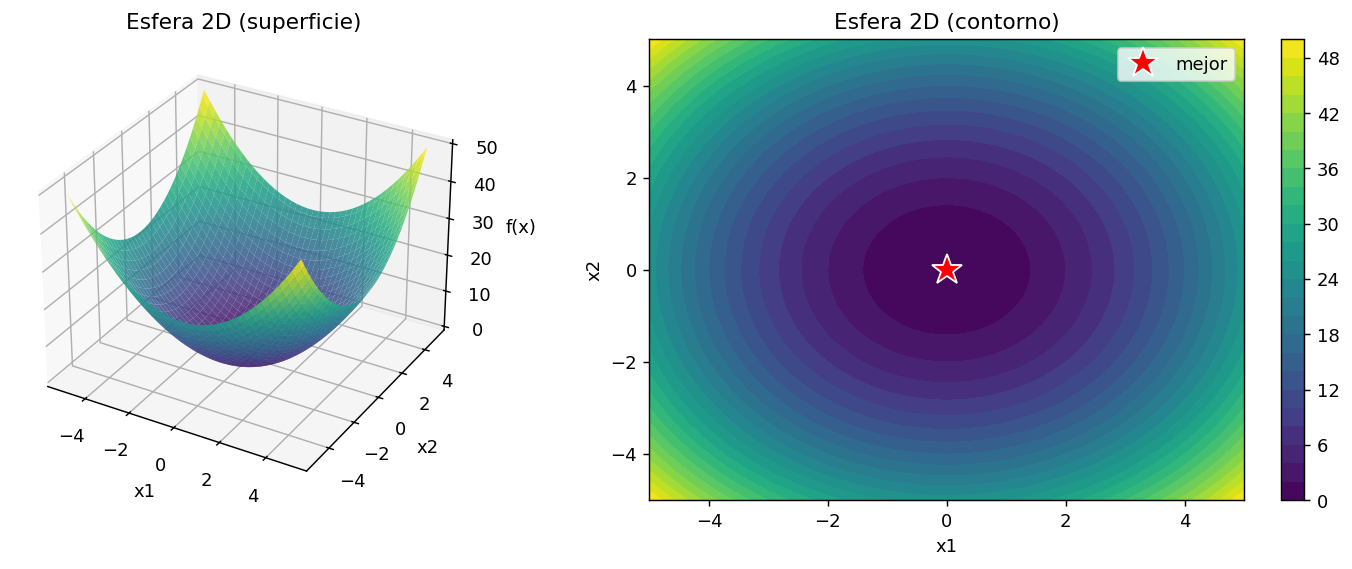
\includegraphics[width=14cm]{figs/AG_min_esfera.png}
\caption{Minimizaci\'on de la funci\'on Esfera. La estrella roja marca la mejor soluci\'on encontrada por el AG.}
\end{figure}

\subsubsection{Funci\'on de Rastrigin}

Funci\'on altamente multimodal con m\'inimo global en $\mathbf{x}^* = (0,0)$. El AG localiza la regi\'on del \'optimo global: mejor soluci\'on $(-8\times10^{-5},\,8\times10^{-5})$, $f = 2.42\times10^{-6}$.

\begin{figure}[H]
\centering
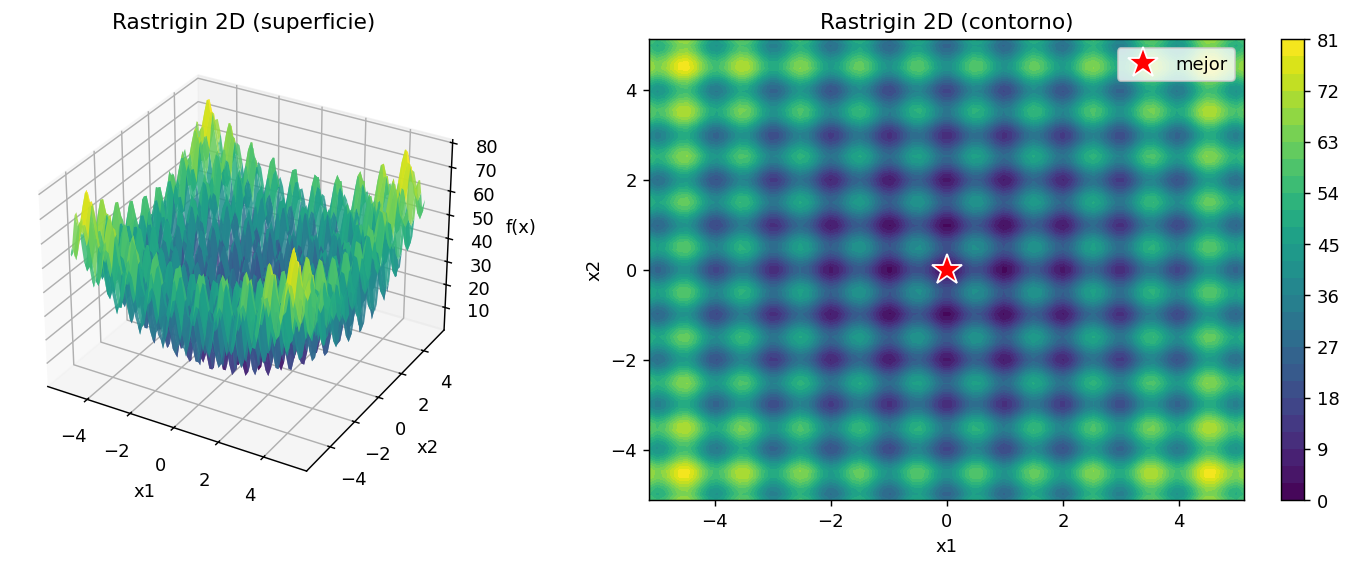
\includegraphics[width=14cm]{figs/AG_min_rastrigin.png}
\caption{Minimizaci\'on de la funci\'on de Rastrigin. La topolog\'ia de valles peri\'odicos requiere que la poblaci\'on mantenga diversidad durante la exploraci\'on.}
\end{figure}

\subsubsection{Funci\'on de Rosenbrock}

Valle curvo estrecho con m\'inimo global en $\mathbf{x}^* = (1,1)$. El AG navega el valle correctamente: mejor soluci\'on $(0.99803,\,0.99614)$, $f = 4.40\times10^{-6}$.

\begin{figure}[H]
\centering
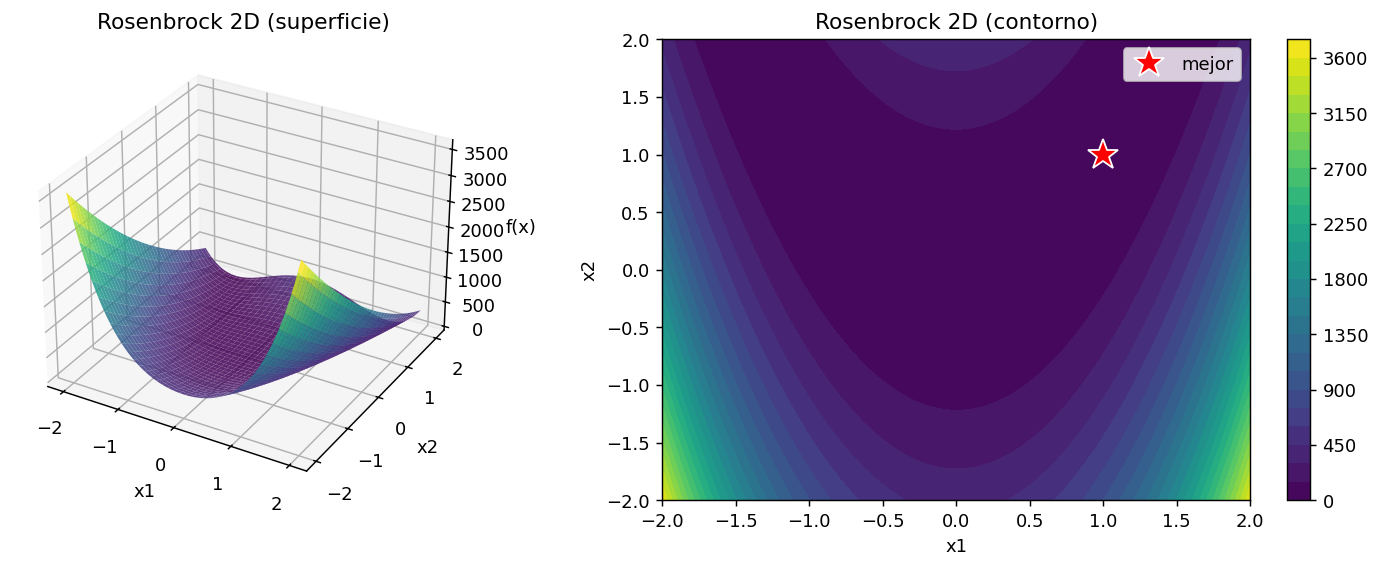
\includegraphics[width=14cm]{figs/AG_min_rosenbrock.png}
\caption{Minimizaci\'on de la funci\'on de Rosenbrock. La superficie en forma de pl\'atano curvado exige que la poblaci\'on siga el valle hasta el m\'inimo.}
\end{figure}

\subsection{Maximizaci\'on 2D}

\subsubsection{Esfera Negativa}

Se maximiza $-f_{\text{esfera}}(\mathbf{x})$, cuyo m\'aximo global es en $(0,0)$. Mejor soluci\'on $(8\times10^{-5},\,8\times10^{-5})$, $f = -1.16\times10^{-8}$.

\begin{figure}[H]
\centering
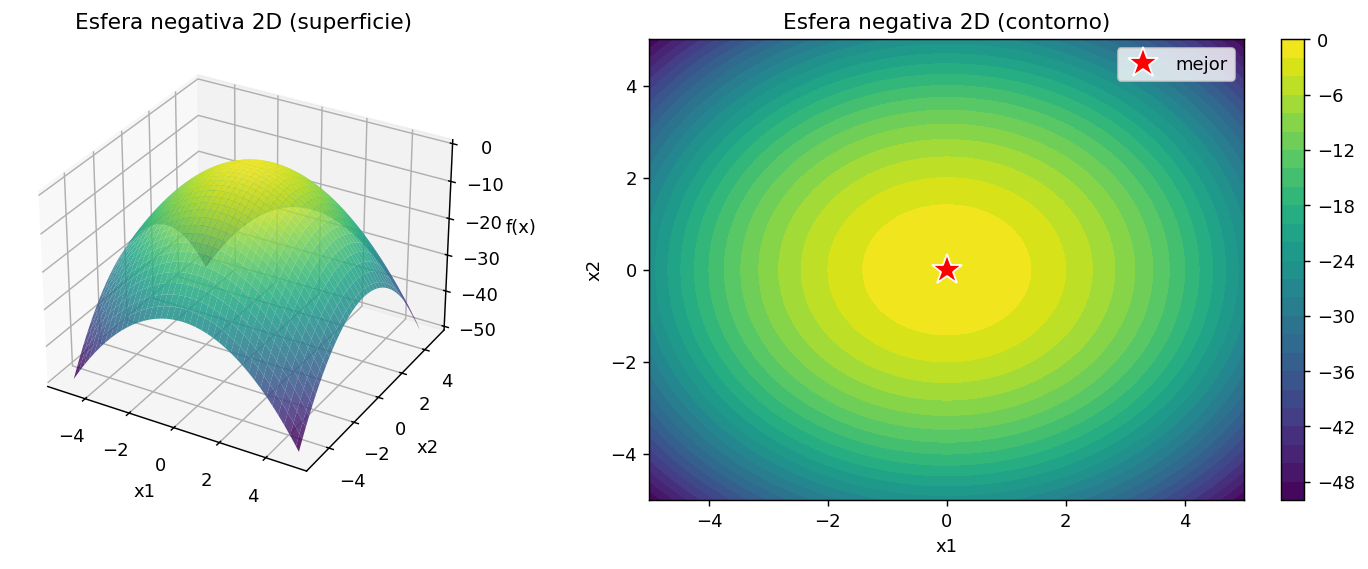
\includegraphics[width=14cm]{figs/AG_max_neg_esfera.png}
\caption{Maximizaci\'on de la esfera negativa. La poblaci\'on converge al punto de m\'aximo de la superficie invertida.}
\end{figure}

\subsubsection{Funci\'on Seno-Coseno}

$f = \sin(x_1)\cos(x_2)$ tiene m\'aximo global de $1.0$ en $(\pi/2,\,0)$ y puntos sim\'etricos. El AG encuentra: mejor soluci\'on $(1.57077,\,5\times10^{-5})$, $f \approx 1.0$.

\begin{figure}[H]
\centering
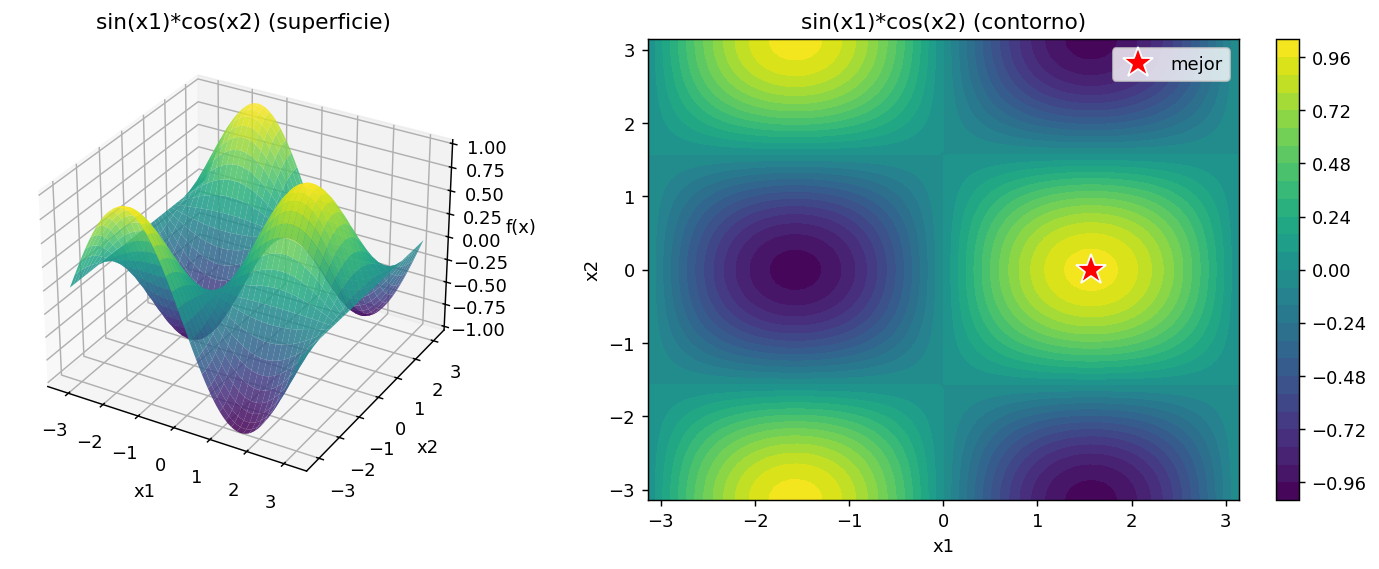
\includegraphics[width=14cm]{figs/AG_max_seno_coseno.png}
\caption{Maximizaci\'on de $\sin(x_1)\cos(x_2)$. La funci\'on presenta m\'ultiples m\'aximos id\'enticos; el AG localiza uno de ellos con valor $f \approx 1$.}
\end{figure}

\subsubsection{Funci\'on Easom}

M\'aximo global en $(\pi,\,\pi)$ con $f = 1.0$. La funci\'on es casi cero en casi todo el dominio, lo que dificulta la orientaci\'on de la poblaci\'on. Mejor soluci\'on $(3.18755,\,3.14058)$, $f = 0.9968$.

\begin{figure}[H]
\centering
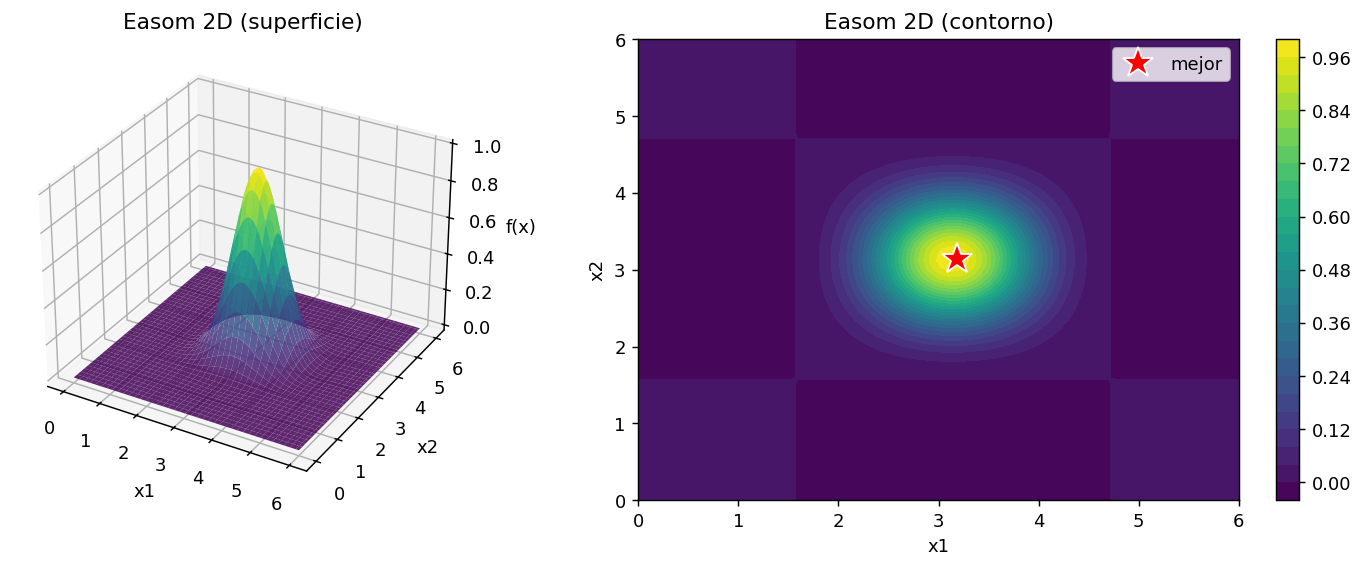
\includegraphics[width=14cm]{figs/AG_max_easom.png}
\caption{Maximizaci\'on de Easom. El pico estrecho en $(\pi,\pi)$ requiere explorar un dominio mayoritariamente plano antes de localizar el m\'aximo.}
\end{figure}

\subsection{Minimizaci\'on N-Dimensional (4D)}

\begin{table}[H]
\centering
\begin{tabular}{lp{8.5cm}r}
\hline\hline
Funci\'on & Mejor soluci\'on & $f(\hat{\mathbf{x}})$ \\
\hline
Esfera    & $[-8{\times}10^{-5},\;8{\times}10^{-5},\;-8{\times}10^{-5},\;-8{\times}10^{-5}]$ & $2.33\times10^{-8}$ \\[3pt]
Rastrigin & $[-8{\times}10^{-5},\;8{\times}10^{-5},\;-8{\times}10^{-5},\;-8{\times}10^{-5}]$ & $4.84\times10^{-6}$ \\[3pt]
Ackley    & $[-4.9{\times}10^{-4},\;-4.9{\times}10^{-4},\;4.9{\times}10^{-4},\;4.9{\times}10^{-4}]$ & $1.97\times10^{-3}$ \\
\hline\hline
\end{tabular}
\caption{Resultados de minimizaci\'on en 4 dimensiones. Las tres funciones convergen al \'optimo global con alta precisi\'on num\'erica.}
\end{table}

\subsection{Maximizaci\'on N-Dimensional (4D)}

Se maximizan las versiones negadas de las funciones anteriores.

\begin{table}[H]
\centering
\begin{tabular}{lp{8.5cm}r}
\hline\hline
Funci\'on & Mejor soluci\'on & $f(\hat{\mathbf{x}})$ \\
\hline
$-$Esfera    & $[-8{\times}10^{-5},\;-8{\times}10^{-5},\;-8{\times}10^{-5},\;-8{\times}10^{-5}]$ & $-2.33\times10^{-8}$ \\[3pt]
$-$Rastrigin & $[-8{\times}10^{-5},\;8{\times}10^{-5},\;8{\times}10^{-5},\;-8{\times}10^{-5}]$   & $-4.84\times10^{-6}$ \\[3pt]
$-$Ackley    & $[-4.9{\times}10^{-4},\;-4.9{\times}10^{-4},\;4.9{\times}10^{-4},\;-4.9{\times}10^{-4}]$ & $-1.97\times10^{-3}$ \\
\hline\hline
\end{tabular}
\caption{Resultados de maximizaci\'on en 4 dimensiones. El comportamiento es sim\'etrico al de minimizaci\'on.}
\end{table}

\section{Conclusi\'on}

El AG con codificaci\'on binaria encontr\'o el \'optimo global en funciones unimodales (Esfera, Rosenbrock) y cuasiunimodales (Ackley) tanto en 2D como en 4D con alta precisi\'on. En 2D logr\'o los m\'aximos exactos de Seno-Coseno y Easom. En 4D las tres funciones convergieron al \'optimo global, lo que confirma la efectividad del algoritmo en espacios de b\'usqueda de dimensi\'on moderada.\\\\
La precisi\'on de la soluci\'on est\'a acotada por la resoluci\'on de la codificaci\'on binaria: con $b = 16$ bits por dimensi\'on, la distancia m\'inima entre dos valores representables es $(\ell_{\max}-\ell_{\min})/(2^{16}-1) \approx 1.5\times10^{-4}$, lo que explica que las soluciones \'optimas aparezcan como m\'ultiplos de $\approx 8\times10^{-5}$.\\\\
El elitismo garantiza que la aptitud no retrocede entre generaciones, acelerando la convergencia. Sin embargo, puede reducir la diversidad y favorecer la convergencia prematura en funciones muy multimodales como Rastrigin. La selecci\'on por torneo con $k=3$ equilibra presi\'on selectiva y diversidad sin requerir c\'alculo de probabilidades acumuladas como en la ruleta.

\end{document}
